\begin{frame}{}
    \LARGE Generative AI for Science: \textbf{Climate Simulation}
\end{frame}

\begin{frame}[allowframebreaks]{Climate Simulation}
    \begin{figure}
        \centering
        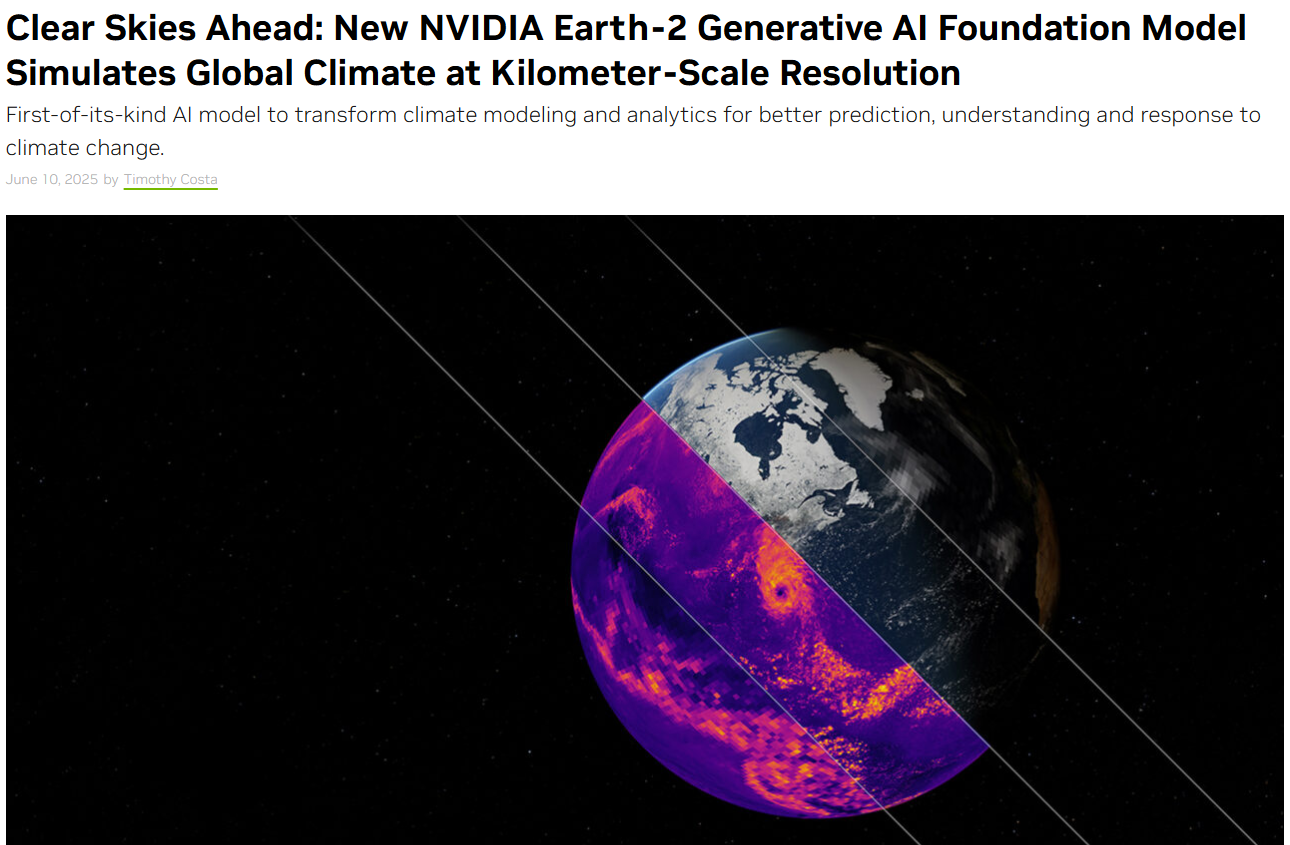
\includegraphics[height=0.9\textheight,width=1\textwidth,keepaspectratio]{images/science/climate-sim-cover.png}
    \end{figure}

    \framebreak

    \textbf{Applications of Generative AI in Climate Simulation}
    \begin{itemize}
        \item \textbf{High-Resolution Climate Modeling:} Generative AI enables kilometer-scale global climate simulations, providing much finer detail than traditional models.
        \item \textbf{Faster Simulations:} AI-driven models can generate climate predictions much faster, supporting rapid scenario analysis and decision-making.
        \item \textbf{Extreme Weather Prediction:} Enhanced resolution and speed help in forecasting extreme weather events, such as hurricanes and floods, with greater accuracy.
        \item \textbf{Data Gap Filling:} AI models can fill in missing observational data, improving the completeness and reliability of climate datasets.
        \item \textbf{Scenario Exploration:} Researchers can quickly test the impact of different interventions or policy decisions on future climate outcomes.
        \item \textbf{Support for Climate Research and Policy:} These advances empower scientists and policymakers with better tools for understanding climate risks and planning mitigation strategies.
    \end{itemize}

    \framebreak

    \begin{figure}
        \centering
        \href{https://build.nvidia.com/nvidia/fourcastnet?snippet_tab=Try}{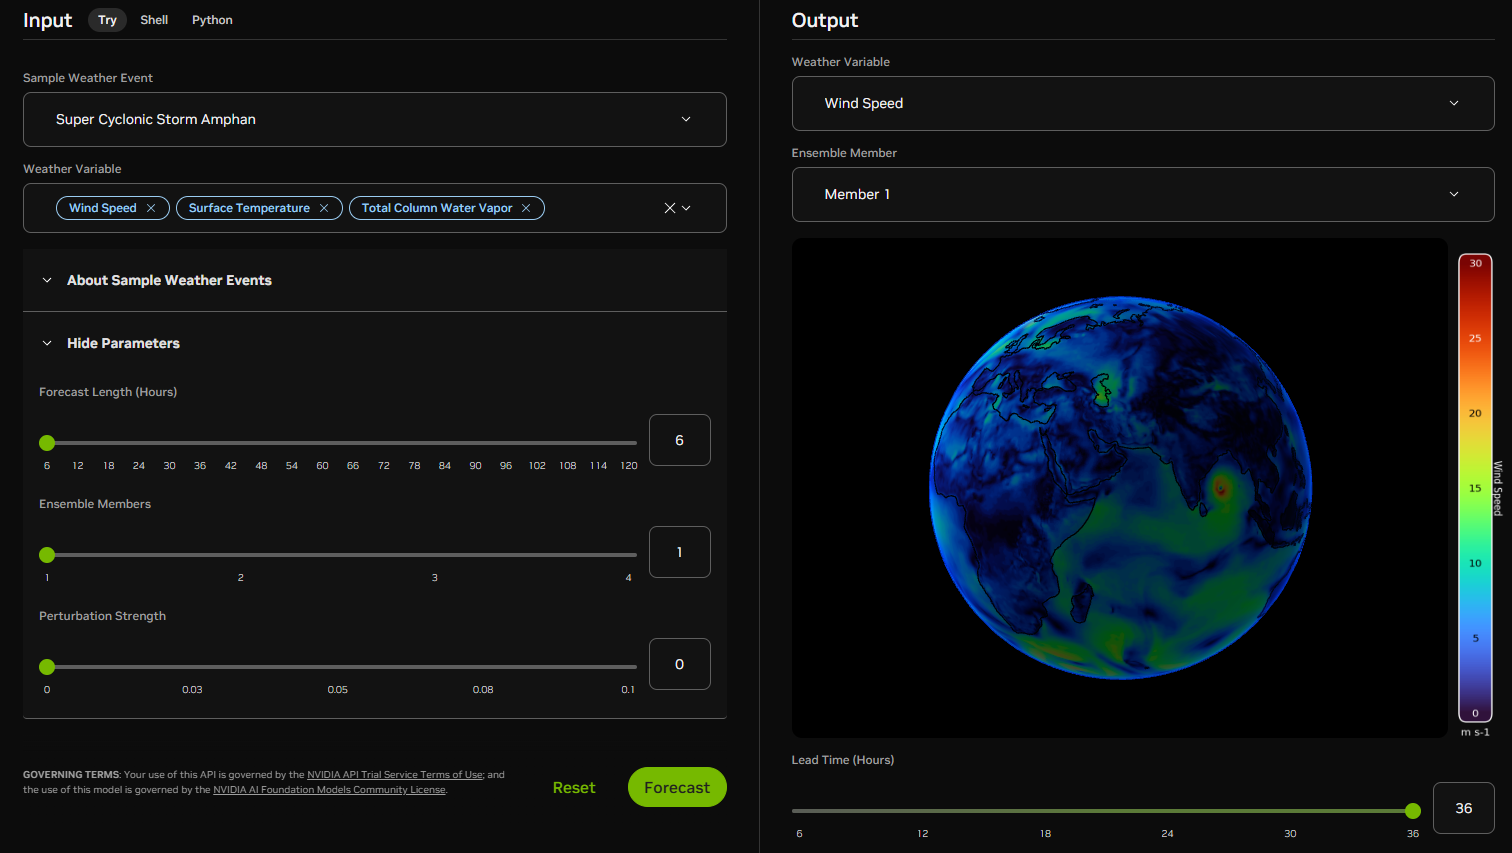
\includegraphics[height=0.9\textheight,width=1\textwidth,keepaspectratio]{images/science/climate-sim-nvidia-1.png}}
    \end{figure}

    \framebreak

    \begin{figure}
        \centering
        \href{https://build.nvidia.com/nvidia/fourcastnet?snippet_tab=Try}{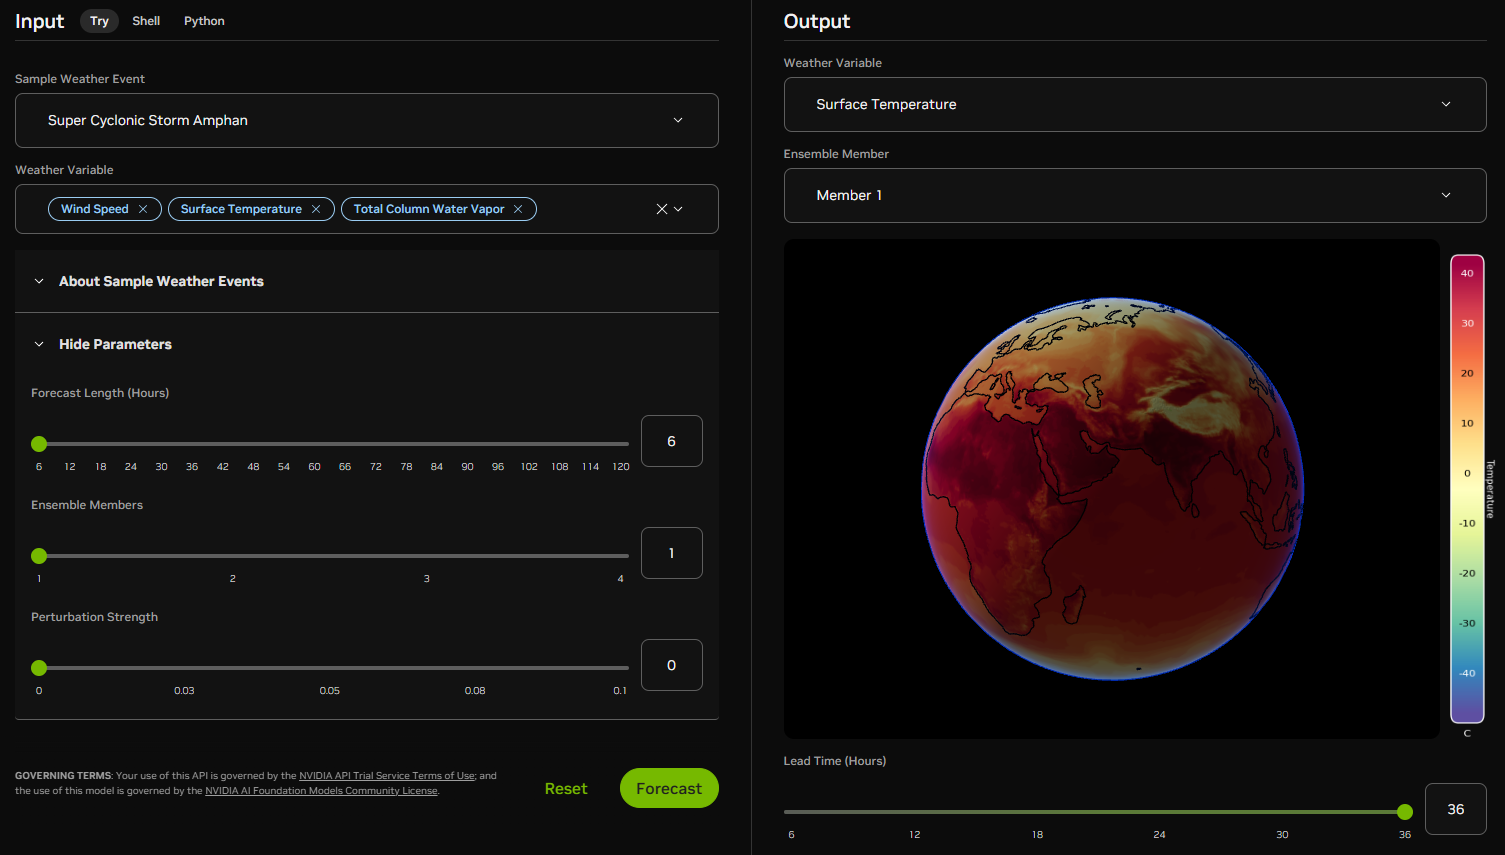
\includegraphics[height=0.9\textheight,width=1\textwidth,keepaspectratio]{images/science/climate-sim-nvidia-2.png}}
    \end{figure}

    \framebreak

    \begin{figure}
        \centering
        \href{https://build.nvidia.com/nvidia/fourcastnet?snippet_tab=Try}{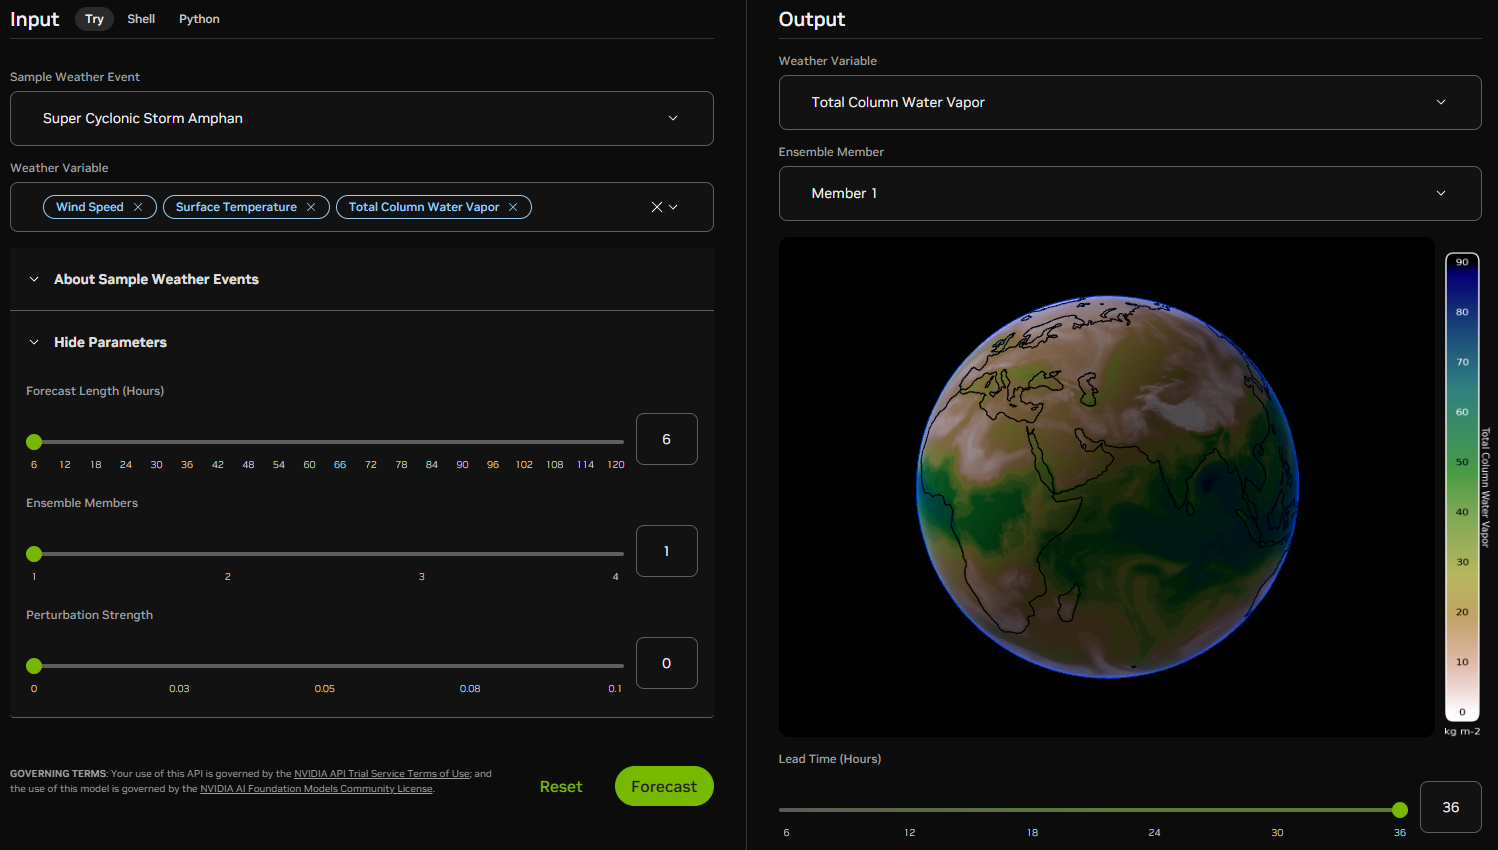
\includegraphics[height=0.9\textheight,width=1\textwidth,keepaspectratio]{images/science/climate-sim-nvidia-3.png}}
    \end{figure}

    \framebreak

    \begin{center}
        \href{https://build.nvidia.com/nvidia/fourcastnet?snippet_tab=Try}{\texttt{nvidia/fourcastnet}}
    \end{center}

    \framebreak

    \begin{figure}
        \centering
        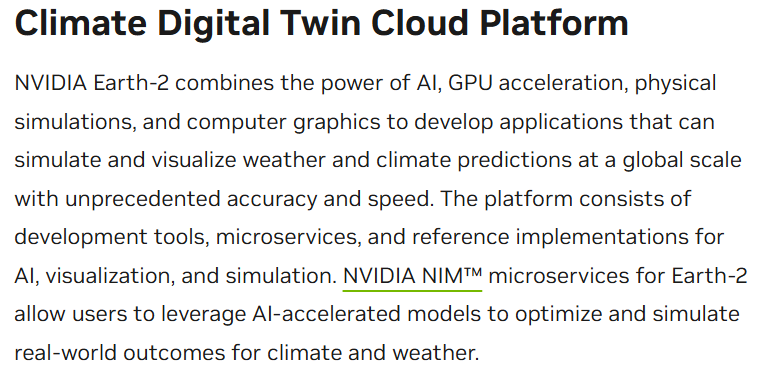
\includegraphics[height=0.9\textheight,width=1\textwidth,keepaspectratio]{images/science/climate-sim-earth-2.png}
    \end{figure}

    \framebreak

    \textbf{NVIDIA Earth-2 Platform}

    \begin{itemize}
        \item \textbf{Overview:} Earth-2 is NVIDIA’s platform for kilometer-resolution global climate simulations, leveraging GPU acceleration and scalable microservices architecture.
        \item \textbf{Key Features:}
        \begin{itemize}
            \item High-performance, real-time climate modeling.
            \item Modular microservices for flexible deployment.
            \item Integration with advanced generative AI models.
        \end{itemize}
        \item \textbf{Use Cases:}
        \begin{itemize}
            \item \textbf{NOAA Adoption:} Used by the National Oceanic and Atmospheric Administration for advanced weather and climate forecasting.
            \item \textbf{Digital Twin Demonstrations:} Enables creation of digital twins of the Earth for scenario analysis and visualization.
        \end{itemize}
    \end{itemize}

    \framebreak
    \textbf{Latest Advances: cBottle \& CorrDiff}

    \begin{itemize}
        \item \textbf{Climate in a Bottle (cBottle):}
        \begin{itemize}
            \item 5 km resolution global climate model designed to provide actionable insights for policymakers.
            \item Enables rapid scenario analysis and supports climate-related decision-making.
            \item See: \href{https://climatesciencefair.emersoncollective.com}{climatesciencefair.emersoncollective.com}
        \end{itemize}
        \item \textbf{CorrDiff:}
        \begin{itemize}
            \item Ultra-high-resolution local weather forecasting using generative AI.
            \item Delivers detailed, accurate predictions for specific regions and extreme events.
        \end{itemize}
    \end{itemize}

    \begin{center}
        \href{https://www.youtube.com/results?search_query=climate+in+a+bottle}{\texttt{youtube.com: Climate in a Bottle}}
        \hspace{1cm}
        \href{https://www.youtube.com/results?search_query=CorrDiff}{\texttt{youtube.com: CorrDiff}}
    \end{center}

    \framebreak

    \textbf{Limitations and Challenges}

    \begin{itemize}
        \item \textbf{Uncertainty Propagation:} Generative AI models may not fully capture or propagate uncertainties inherent in climate systems, which is critical for robust scientific predictions.
        \item \textbf{Data Assimilation:} Integrating real-time observational data into AI-driven simulations remains a significant challenge, limiting model adaptability and accuracy.
        \item \textbf{Cost and Trust:} High computational costs and the need for rigorous validation can hinder adoption. For example, models like CorrDiff are still under testing and not yet fully trusted for operational use.
        \item \textbf{Interpretability:} Understanding the decision-making process of complex AI models is difficult, which can impact scientific transparency and acceptance.
    \end{itemize}

\end{frame}